\documentclass[
a4paper 
%, man
, doc
%, jou
%, draftfirst 
, longtable
]{apa6} 
\usepackage{rotating} 
                          % use this in jou and doc modes only, with \sideways. 
                          % In man mode use the documentclass option longtable and do not load rotating.
\usepackage{csquotes}  
\usepackage[american]{babel}                     
\usepackage[style=apa, sortcites=true, sorting=nyt, backend=biber, doi=false, isbn=false]{biblatex}
    \DeclareLanguageMapping{american}{american-apa}
    \addbibresource{vcr.bib}
\usepackage{datetime}
\usepackage{url}

                         %% OTHER DOCUMENTCLASS OPTIONS 
                         % floatsintext (in man mode do not flush floats, better for internal reading, 
                         %                    but do not use for submission to journals)
                         % mask (masks references that are marked as self-references, for blind peer review)
                         % longtable (in man mode only)
                         % notxfonts (in jou mode suppresses txfonts in case pslatex or times is preferred)
                         % notimes (in jou mode use Computer Modern instead of loading txfonts or pslatex or times)
                         % notab (in jou mode suppress auto stretching of tabular environments to fill their float)
                         % helv (in man mode use Helvetica instead of Computer Modern)
                         % tt (in man mode use typewriter font)
                         % draftfirst or draftall (places the word DRAFT on first page or all pages)
                         % draft (is passed to, and handled by, the article documentclass)

%\SetWatermarkAngle{0} % Angle at which the watermark text is drawn
%\SetWatermarkColor{red} % Color of the watermark
%\SetWatermarkLightness{0.7} %Lightness of the watermark text (1=white, 0=black)
%%\SetWatermarkFontSize{?length?} Font size of the watermark text
%\SetWatermarkScale{0.5} % Scaling of the watermark text 
%%\SetWatermarkHorCenter{?length?} Horizontal center of watermark text 
%\SetWatermarkVerCenter{2cm} % Vertical center of watermark text
%\SetWatermarkText{Internal Draft} %Watermark text

\title{Vagueness as Cost Reduction}
\shorttitle{Vagueness as Cost Reduction}
\twoauthors{Matt Green}{Kees van Deemter}
\leftheader{Green, van Deemter} % for even-page headers in jou mode
\twoaffiliations{Computing Science\\ University of Aberdeen}{Computing Science\\ University of Aberdeen}
\abstract{Much of everyday language is vague, yet standard game-theoretic models make it difficult to see how vague expressions can have benefits over crisp ones in co-operative situations. We report a series of experiments that aims to separate the utility of vagueness from the utility of other factors that come together with vagueness. We argue that the results support a view of vagueness where the benefits that vague terms exert are due to other influences that vagueness brings with it rather than to vagueness itself.}
\keywords{keyword 1, keyword2, keyword3, keyword4}
\authornote{Contact author is Matt Green: \textsf{mjglab@gmail.com}} 
% The Author Note, containing contact information, acknowledgements, etc.
\note{This version compiled at: \textsf{\currenttime~\today}} 
% Notation of manuscript date or other information desired beneath affiliation line
\journal{Aimed at:}
% typeset in the top left header of page 1 (jou and doc modes only)
\volume{\textsc{Language, Cognition, and Neuroscience}} 
% Volume, number, pages; typeset in the top left header in jou and doc modes, underneath the content of \journal
\ccoppy{Draft date:}
% Copyright notice, etc.; typeset in the top right header of page 1 (jou and doc modes only)
\copnum{\today}
% Any additional text needed;  typeset in the top right header in jou and doc modes, underneath the content of \ccoppy
\begin{document}
\longdate
\maketitle % no blank line
%\section{Introduction} % APA does not use Introduction header
Vagueness pervades the language that we use on a daily basis. In everyday use, language use may be called vague for various reasons (see e.g. the entry ``vague'' in \cite{penguin}.) 
In most academic use though, the word `vagueness' has a more particular meaning. Keefe and Smith, for example, state ``vague predicates have borderline cases, have fuzzy boundaries, and are susceptible to sorites paradoxes'' \cite[p.\ 4]{keefe1997vagueness} (a similar definition can be found in \textcite{EgreKlinedinst}, among many others).  The most crucial of these criteria is the existence of borderline cases: ``a word is precise if it describes a well-defined set of objects. By contrast, a word is vague if it is not precise'' \cite[p.\ 1]{lipmanvague}. A typical example is the word ``tall'', as applied to people for example, because here is no precise, known height which separates those who are tall from those who are not. The crucial point is that ``tall'' admits borderline cases (i.e., people who may or may not count as tall), which are the hallmark of vagueness as we use the term.

Linguists, philosophers of language, and more recently game theorists, have asked why natural languages contain so many vague expressions, which are used so frequently \cite{Lipman:2000fk, lipmanvague}. By introducing borderline cases, these expressions create potential misunderstandings, thereby creating ``a worldwide several-thousand year efficiency loss'' \cite[][p.~1]{lipmanvague}. Lipman explains the point by means of a scenario in which a speaker describes a person to a hearer, who needs to identify that person in the arrivals hall of of an airport. Lipman argues that, in such a scenario, a precise description of the person's height (e.g., ``The person's height is 187.96 cm'') would be more useful than a vague one (``The person is tall''). Lipman uses this scenario to explain why standard game theory models of communication \cite[e.g.,]{Crawford:1982lr} predict that, under certain conditions, a crisp act of communication will always have more utility than a vague act that communicates the same state of affairs. The relevant conditions are, broadly speaking, that both interlocutors know all the relevant facts (e.g., both know the person's height precisely) and that the setting for the communication is co-operative. These conditions exclude deliberate deception, and rhetorical situations like political debate and advertising where the intention is to persuade the interlocutor to adopt some point of view, where the persuasion might not be intended to be in the addressee's best interest. 

Lipman argued that such the efficiency loss resulting from vague expressions would be unlikely to have arisen unless there are advantages as well as disadvantages associated with vague expressions. Lipman asked, essentially, what these advantages might be, and how they might find a place in a game-theoretical explanation. In this paper, we focus on the first part of Lipman's question.

Several tentative answers to Lipman's question have been offered  \parencite[see][]{van2009utility, van2010vagueness}. Prominent among these answers is the idea that vague expressions are somehow easier to process, by a speaker and/or a hearer, than expressions that are not vague (i.e., crisp) \cite[e.g.,][]{lipmanvague,De-Jaegher:2003lr,vanrooij2003lr}. For example, \textcite[][p.\ 11]{lipmanvague} writes: ``For the listener, information which is too specific may require more effort to analyze''. We shall refer to this characterisation of the utility of vague language as the \emph{cost reduction} hypothesis. The idea of vagueness as cost reduction can take various shapes, but the basic hypothesis is that it is easier for people to think in terms of loosely defined categories (such as ``quite a few'', or ``many'') than in terms of crisply defined ones (such as ``thirteen'', or ``237''). This predicts that whenever a vague expression can perform the same communicative task as a precise one, it is rational to choose the vague expression. The corollary for comprehension is that vague expressions should be understood more readily than precise expressions. 

Questions concerning optimal language use have many practical applications. Natural Language Generation\footnote{NLG systems take data or formulas as input, and transform them into natural language outputs \cite[][]{reiter2000building}. The process parallels language production in humans.}  (henceforth NLG) systems must make decisions between different formulations of the same information. For example, if a man's height is 6 foot 2 inches, this could be expressed as ``187.96 metres'', ``6 foot 2'', or ``tall'', among other ways, and the NLG system must decide between these.  The problem is particularly relevant for NLG systems that take numbers as input, as many do. In the context of an NLG system faced with a practical decision of this kind, Lipman's question becomes ``Under what circumstances should vague terms be produced?''  Relevant applications include weather forecasting on the basis of numerical weather data such as temperature and wind speed \cite{goldberg1994using,turner2006generating}, and medical decision support on the basis of clinical measurement such as oxygen saturation, heart rhythm, etc. \cite{Hripcsak01032009, hunter2008summarising, portet2009automatic}. At present, such NLG systems are often forced to make decisions concerning the level of precision in the utterances that they generate (e.g., ``the temperature will be in the high twenties tomorrow'') on the basis of little more than intuition. A better understanding of the benefits of different precision levels for readers would allow these systems to become more useful. 

The cost reduction hypothesis is of direct relevance to psycholinguists interested in language comprehension, and additionally to psycholinguists interested in language production, for example in connection with the question of audience design \cite{Clark1982287}. For, to the extent that speakers and writers choose vague expressions over and above crisp ones because the former are easier to process for hearers than the latter, the cost reduction hypothesis suggests that speakers design their utterance for optimal benefit to their hearers -- out of altruism, so to speak.

The utility of vagueness is the attested aim of a small number of studies, but most of these have focussed on vagueness in a different sense, and focussing on different types of benefits for hearers. Two recent studies can illustrate both issues. 

In a series of studies of behaviour modification, \textcite[]{Mishra01042011} manipulated the presentation format of information about quantities in the domains of mental acuity, physical strength, and weight loss. In the weight loss study, participants were told that the study was designed to test the validity of a new (actually fictitious) health index, the HHI (Holistic Health Index). They were told that an ideal HHI score lies in the range of 45 to 55. In a longitudinal study, participants submitted their height, weight, hydration level, gender, and age to a computer each week. Participants were told that two algorithms would be used to compute their HHI, and that it was possible that the two algorithms might give different values initially, but would converge over the course of the study to a single value. They were also told that if the two algorithms did give different values, then the true score lay between the two values. In one condition, which the authors called the precise condition, the two algorithms gave the same score. In the other condition, which the authors called the vague condition, one algorithm added 3\% to the score while the other algorithm subtracted 3\% from the score, yielding a range of values whose midpoint was the same as the two values given in the precise condition. 

One group of participants was given HHI scores in the ideal range: for this group their weight loss did not differ depending on whether they were given vague or precise HHI values. However for the other group, who were given HHI scores outside the ideal range, their weight loss was significantly greater if they were given vague HHI scores than if they were given precise HHI scores. The authors explain the improvement in the vague condition for this group as resulting from the participants' freedom to think of themselves a positioned on one end of the range - the end closest to the ideal HHI scores. This ``illusion of proximity'' \cite[][p.~4]{Mishra01042011} to the goal is argued to allow participants to generate positive expectancies that lead to behaviours that improve performance. In contrast, in the precise conditions, participants did not have this freedom of interpretation, and could not distort the information to bring about the beneficial \emph{illusion of proximity}. These results are interesting, and of obvious potential practical importance. We note, however, that information presented as an exact range of values does not conform with the standard definition of vagueness \cite{keefe1997vagueness, EgreKlinedinst}, since an exact range does not admit borderline cases. In the terminology of \textcite{Hobbs85granularity}, the difference between a range and a single midpoint value is a difference of \emph{granularity}. Furthermore, the experiments of \textcite{Mishra01042011} did not explore benefits in terms of processing cost, but in terms of long-term behaviour change.

Similar issues arise from the work of \textcite{peters2009bringing}. The authors carried out a series of studies where participants were required to rate hospitals based on various sources of information about quality of care. There was a between-subjects manipulation based on numeracy. The format of the information was manipulated within subjects: either numbers only were presented, or both numbers and evaluative categories were presented (e.g., \emph{Poor}, \emph{Fair}, \emph{Good}, \emph{Excellent}, with crisp visual boundary lines between the categories). Results showed that, for low-numeracy participants, the presence of evaluative categories resulted in a diminished influence of an irrelevant affective state on the ratings. For all participants, the presence of evaluative categories resulted in better decisions and in a greater use of the most important and reliable types of information, such as survival rates. 

It is, however, questionable whether the ``evaluative categories" manipulation in this study can be considered a manipulation of vagueness. Certainly, terms like \emph{Fair} admit the possibility of borderline cases. However, given that the boundaries between the categories were marked crisply, and that therefore the categories mapped crisply to numerical values, it becomes doubtful whether any borderline cases could be conceived to arise in fact. For example, \emph{Fair} was mapped to 60\% -- 70\% for the variable \emph{percentage of heart attack patients given recommended treatment (ACE inhibitor)}. Accordingly, rather than the vagueness of categories such as \emph{Poor}, Peters et al. emphasise the evaluative content inherent in these categories, and the affective potential of the evaluative content rather than the vagueness of the terms like {\em Fair}.
%\\[2ex]
\subsection{}
The experiments reported in the present paper put the cost reduction hypothesis to the test. The question that we are trying to answer is whether vague expressions are processed more easily by readers than crisp ones. Like Lipman, we focus on situations where numerical information is used in order to identify a referent. Reference, in other words, will be the linguistic task on which we focus, partly because of the interest that this topic has recently drawn from the NLG community.  In focussing on benefits for the hearer, we will leave aside the question of audience design, leaving this for later research.

In using references to quantities to test the cost reduction hypothesis we are only testing one aspect of vagueness in a particular context. This limits the applicability of our results. It also has the advantage that we can explore the costs and benefits of vagueness more thoroughly in that context. Since one prevalent view of vagueness is that a vague expression is never preferable to a crisp equivalent, a demonstration of a benefit for vagueness in any context would advance the discussion.

In our experiments we used a speeded forced choice task to compare the processing costs of different references to quantities. In this context, speed and accuracy of responses are the key dimensions on which the different references can be compared. The stimuli in the experiments were sets of dot arrays containing various numbers of dots. The forced choice was to identify one dot array given a reference to a given quantity of dots. We manipulated the references in several ways across a series of four experiments. 

Our main manipulation was always of vagueness: we constructed crisp and vague versions of references to the same dot array. For example, in experiment 1 the instruction presented to the participant could be \emph{Choose the square with many dots.} (vague condition), or \emph{Choose the square with 20 dots.} (crisp condition), identifying the same dot array.

Ideally, we would manipulate vagueness independently of other variables. However, in practice, and given the constraints imposed by the use of natural language, any manipulation of vagueness introduces variance along other dimensions as well. Therefore we carried out further experiments to try to address and control variance along other dimensions. 

One non-vagueness source of variance was the difference between numerical and verbal format in the references. For example, in the instructions for experiment 1 given above, \emph{many} is in verbal format (as well as vague) and \emph{20} is in numerical format (as well as crisp). Therefore any difference observed between responses to the \emph{many} instruction and the \emph{20} instruction could be due either to vagueness or to {\bf instruction format}. It is possible to create vague and crisp references in each of these instruction formats: for example in numerical instruction format we can have \emph{20} (crisp) and \emph{about 20} (vague), and in verbal instruction format we can have \emph{the most} (crisp) and \emph{many} (vague). Experiment 2 varied vagueness and instruction format factorially in a similar way to this, to try to tease apart these two sources of variance.

Another potential non-vagueness source of variance between responses to the \emph{many} (verbal vague) references and the \emph{20} (numeric crisp) references lies in the method used to identify a referent (we call this the {\bf selection algorithm} source of variance). Identifying the array with \emph{many} dots might be done by a \emph{comparison} algorithm, identifying that one array is more numerous than the others without establishing the numerosity of any arrays, whereas identifying the array with \emph{20} dots, which might be done by a \emph{matching} algorithm would require an estimate of the numerosity of the arrays. It seems reasonable that comparison would be faster than matching because it does not require estimates of cardinality. Furthermore the problem persists when using references like \emph{the most} (verbal crisp) and \emph{about 20} (numeric vague), since they too vary not only along the vague/crisp dimension and the numeric/verbal dimension but also along the comparison/matching dimension. Experiments 3 and 4 addressed the \emph{selection algorithm} source of variance - experiment 3 crossed vague/crisp and comparison/matching factorially using only numerical references, and experiment 4 crossed vague/crisp and comparison/matching factorially using only verbal references.  

\section{Experiment One} 

\subsection{Introduction}
We used a forced choice task to compare choices made in response to vague instructions against choices made in response to crisp instructions. The participant was presented with an instruction like ``Choose the square with many dots'' in the vague conditions, or ``Choose the square with 20 dots'' in the crisp conditions. Then two dot arrays were presented in the form of squares containing a number of dots. Fig \ref{stimuluse1} shows an example stimulus. The participant was required to identify the square that corresponded with the instruction, by pressing the appropriate key.
Response time and accuracy were recorded for analysis. 

Our main manipulation was of the vagueness of the instruction, with two levels, vague and crisp. Table \ref{instructionse1} shows examples from each condition.  We also manipulated how discriminable the dot arrays were. One array always contained 25 dots: the other contained either 5, 10, 15, 20, 30, 35, 40, or 45 dots. This led to numerical differences of 5, 10, 15, and 20, with lower differences resulting in less discriminable arrays and larger differences representing more discriminable arrays. There is evidence that when the distance grows between two numbers, they become more easily distinguishable from each other: the \emph{numerical distance effect}, which has been shown for comparing the numerosity of two sets of dots \cite{van123} and for processing Arabic numerals and number words \cite{Dehaene199647}. Where a number was mentioned in the instruction, it was always in the form of an Arabic numeral.

The instructions indicated the larger of the two dot arrays equally often as they indicated the smaller of the dot arrays, so that participants could not systematically choose the larger or smaller array as a successful response strategy. There is evidence that when two numbers are presented with the smaller on the left, this left-side presentation facilitates responses indicating the smaller number: the \emph{Spatial-Numerical Association of Response Codes (SNARC)} effect \cite{dehaene1993mental, gevers2006automatic}. We controlled which side the smaller number appeared on to avoid systematic influences of this effect. 

\begin{table}[htbp]
\caption{Table of instructions for the pair (5,25). Experiment 1}
\label{instructionse1}
\begin{tabular}{rl}
\toprule
vagueness&example\\
\midrule
crisp 	& 	Choose the square with 5 dots \\
vague	&	Choose the square with few dots\\
\bottomrule
\end{tabular}
\end{table}

\subsection{Hypotheses}
The {\bf cost reduction} hypothesis predicts that responses will be faster and more accurate for the vague conditions than for the crisp conditions because the vague conditions impose a lower cognitive load than the crisp conditions. 

The {\bf instruction format} hypothesis predicts that responses will be faster and more accurate in the vague (i.e., verbal) conditions than in the crisp (i.e., numerical) conditions because numbers are harder to process than verbal references to quantities.

The {\bf selection algorithm} account predicts that responses will be faster and more accurate in the vague (i.e., comparison) conditions than in the crisp (i.e., matching) conditions because it is easier to carry out comparison than matching. 

Thus all three accounts predict a main effect advantage of vagueness, but for different reasons. All three accounts also predict a main effect advantage for greater numerical distance, because greater numerical distances lead to more easily discriminable arrays. The accounts also share the prediction of an interaction effect whereby the main effect advantage of vagueness should diminish as numerical distance increases.

% KvD I'm tentatively starting with a general explanation of the methodology of this group of experiments.

%{\bf General.} All our experiments shared essentially the same methodology: Participants aged between ..., self-reported fluent speakers of English, were recruited by .... and were paid 10 ponds for participating. All had normal, or corrected-to-normal vision. A MacBook ... Stimuli were created ... In all except the last experiment (Experiment 5), items were presented as follows: (...) (IF WE DO ADD THIS GENERAL DESCRIPTION THEN REMOVE THE RELEVANT INFO FROM THE DESCRIPTION OF EACH OF THE INDIVIDUAL EXPERIMENTS.)

\subsection{Method}
Twenty participants were recruited by mailing list and paid ten pounds for participating. Participants were aged between 18 and 45, with a median age of 26. All participants self-reported fluency in English, and had normal, or corrected-to-normal vision. A MacBook Pro laptop computer with a 13 inch screen presented the stimuli to the participants. Stimuli were created and presented using the language GNU Octave \cite{eaton:2002} and the Psychophysics Toolbox extensions \cite{ptbx1, ptbx2}. We needed to control which side the target was presented on. Each pair was presented equally often with with the target on the left, as with the target on the right. We also needed to control whether the target was the smaller or larger number. The items with numbers less than 25 (pairs 1 to 4) formed a group with the smaller number as target and the other items (pairs 5 to 8) formed a balancing group with the larger number as the target number.

The experiment was conducted in a quiet room. On arrival in the room, the participant was told that he or she would be presented with an instruction to choose one of two squares by reference to how many dots it contained. Participants were required to press the space key after reading the instruction. Then there was a central fixation cross for 1000 ms, and a blank screen for 500 ms, followed by the squares and dots (without repetition of the referring expression).  The position of the dots was randomised per-trial. Response time was measured as the latency between the presentation of the dots and squares, and the keypress identifying the decision; in this way, the response times can be separated from time spent reading the instructions, which is important since we are only interested in the former.

The display would stay on screen until the participant responded (there was no timing-out). Participants were asked to respond quickly while avoiding errors. There were 8 practice trials, after which the participant was invited to ask any questions about procedure. After answering these the experimenter left the cubicle for the duration of the experiment. The order in which trials were presented was randomised per-participant. There were 256 trials, presented in 4 blocks of 64 trials each, between which the participant could rest. No feedback was given on correct trials, but there was feedback on error trials in the form of the word ``\textsc{wrong!!}'' which flashed on screen.

\begin{figure}[tbp]
\fitfigure{images/stimuluse1}
\caption{An example stimulus from Experiment 1. First the referring expression was presented (left panel). Then after a keypress, and a fixation cross (not pictured) the squares and dots were presented without repetition of the referring expression (right panel)}
\label{stimuluse1}
\end{figure}

\subsection{Results}

A response was counted as erroneous if the square with the wrong number of dots was chosen (when the instruction contained a number); if the square with the larger number of dots was selected (when the instruction was ``Choose the square with few dots"); or if the square with the smaller number of dots was selected (when the instruction was ``Choose the square with many dots".) % KvD Is this addition defining "erroneous" OK?
RTs for trials with erroneous responses were discarded, leading to the loss of 354 trials from 5120, representing 6.9\% of the trials. The correct response RTs were trimmed at 2.5 standard deviations for each subject, leading to the loss of 160 trials, 3.4\% of the correct responses. Means for response times and error rates are given in Fig. (\ref{resultse2}).
A linear mixed model of RT was built using as independent variables vagueness and gap size and their interaction, with random slopes for vagueness and gap size over participants. Vagueness was sum coded: vague $= -.5$, crisp $= .5$; gap size was Helmert coded. Helmert contrasts compare each level against the mean of the previous levels. Level one of this contrast is gap size 5 compared with gap size 10; level two is the mean of gap size 5 and gap size 10 versus gap size 15; and level three is the mean of gap sizes 5, 10 and 15 versus gap size 20. 
$p$ values were calculated using the R package \emph{lmerTest} \cite{lmerTest}.

RTs were faster for vague instructions ($\beta=.109, se=.022, t=4.9, p<.001$). 
%
RT grew faster as gap size increased: level one $(\beta=-.116, se=.012, t=-9.3, p<.05)$, level 2 ($\beta=-.103, se=.009, t=-11.1, p<.001$) and level three ($\beta=-.082, se=.007, t=-11.0, p<.05$). Since discriminability of the dot arrays is easier for larger gap sizes, discriminability probably underlies this effect. Gap size and vagueness interacted significantly for larger gap sizes when modelling RT. % KvD Is it worth saying how they interacted?
The interactions at the different levels of gap size were: level one: ($\beta=.001, se=.016, t=.03, p=.974$); level two ($\beta=-.039, se=.009, t=-4.460, p<.001$); level three ($\beta=-.043, se=.006,t=-7.0, p<.001$). In the crisp conditions RTs started out much slower than in the vague conditions, at the smallest gap size, but the two conditions converged to very fast times at the largest gap size. There were diminishing returns for vagueness as gap size increased. 

\label{accann}
Error rate data were analysed using a generalized logit mixed model \cite{jaeger2008categorical}, with vagueness and gap size and their interaction as independent variables, and with random slopes for vagueness and gap size over participants. 
%
The effect of vagueness on error rates approached significance, with the vague instructions leading to fewer errors ($\beta=.307, se=.173, t=1.8, p=.077$).
%
Error rates decreased as gap size increased: level one ($\beta=-.585, se=.092, ,z=-6.4, p<.001$), level 2 ($\beta=-.434, z=-5.3,p<.001$) and level three ($\beta=-.250,z=-4.1, p<.001$). 
%
Error rates were greater in the crisp conditions than the vague conditions when gap size was small, and this difference diminished with increasing gap size until it reversed at the biggest gap size.
\begin{figure*}[htbp]
\fitfigure{images/resultse1.pdf}
\caption{Experiment 1 results. }
\label{resultse1}
\end{figure*}

\subsection{Discussion}

Results from experiment 1 were in line with the three main accounts. Responses were faster and more accurate when the instructions were in the vague (or verbal, or comparison) conditions than when they were in the crisp (or numerical, or selection) conditions. The speed and accuracy diminished as the arrays became more easily discriminable, and the advantage for vague (or verbal, or comparison) instructions tailed off as the arrays became more easily discriminable.

The cost reduction hypothesis explains the vagueness advantage by claiming that the vague referring expressions place less cognitive load on the comprehender than the crisp referring expressions. It explains the diminishing returns for vagueness in more-discriminable stimuli by claiming that load is low in both conditions for the easily-discriminable stimuli, and that therefore there is no extra benefit to be had from vagueness in the easily-discriminable stimuli. 

The instruction format hypothesis explains the main effect advantage for the vague instructions by observing that the vague instructions used verbal quantifiers whereas the crisp conditions used numerical quantifiers. Under this account it is avoiding numbers that explains the vagueness advantage main effect. The main effect of numerical distance is explained by assuming that larger distances result in more easily discriminable arrays. The vagueness x numerical distance interaction can be explained by assuming that the numerical quantifiers make the task particularly challenging when the stimuli are less discriminable.

The selection algorithm account explains the main effect advantage of the vague conditions as due to the vague conditions allowing a comparison strategy rather than a matching strategy in the crisp conditions. The main effect of numerical distance is explained by claiming that comparison is easier for more discriminable arrays. The diminishing returns for vagueness as numerical distance grows are explained by claiming that the advantage of being able to use comparison is greater for less discriminable arrays than for more discriminable arrays.

\section{Experiment 2}

\subsection{Introduction}

The main result from experiment 1 was that responses were faster and more accurate for vague instructions than for crisp instructions. This finding can be interpreted in line with three different accounts: the cost reduction account, the instruction format account, and the selection algorithm account. 

In experiment 2 we set out to distinguish between the cost reduction account and the instruction format account, leaving the selection algorithm account for experiments 3 and 4. Contrast an expression from the vague condition: `the square with few dots' with an expression from the crisp condition: `the square with 15 dots'. One difference is that `few' is vague (or at least has the potential for vagueness) and `15' is crisp. Another difference is that `few' is a linguistic, or verbal quantifier while `15' is a numerical quantifier, in the sense that a number is mentioned explicitly. Since these two differences were confounded in Experiment 1, the vagueness advantage finding is vulnerable to an alternative interpretation, that what we saw as a vagueness advantage was in contrast an advantage for the verbal form of the quantifier. In the present experiment 2 we pitted these alternative interpretations against each other in a factorial design. 

In Experiment 1, the participants chose one of two squares. The `vague' quantifiers (e.g., `few') uniquely identified one square. Recall our definition of vague  -- ``a word is precise if it describes a well-defined set of objects. By contrast, a word is vague if it is not precise''.  In the first experiment, the quantifiers in the vague conditions did not really meet this definition. This is because there were no borderline cases of the referent that could make the referent set `not well-defined'. Experiment 2 used three squares so that the vague quantifiers always had more than one possible referent. To enhance the potential for the vague quantifiers to have true vagueness in Experiment 2, we also used indefinite articles in the vague instructions. Thus, instead of the instruction \emph{Choose the square with few dots}, we used \emph{Choose a square with few dots}.

In experiment 2, an item was a referring expression followed by a triple of numbers, representing the number of squares in the left, middle, and right squares. We used four different triples of numbers: (6,15,24); (16,25,34); (26,35,44); (36,45,54). Each triple had the following properties: it comprised three squares (instead of two as in Experiment 1); the central number was always presented in the middle of the three; there were two flanking numbers where one was smaller than the central number and one was bigger. 

There was a numerical and a verbal version of each of the vague and crisp referring expressions. See Table \ref{instructionse2} for examples.
The {\em vague numerical condition}'s referring expression was, on half of the presentations in that condition, ``Choose a square with about 10 dots''. None of the squares displayed contained 10 dots. 10 is slightly closer to 6 than to 15. Therefore the best referent for this referring expression was the square with 6 dots;  the borderline response was the square with 15 dots; and the poorest referent was the square with 24 dots. On the other half of the presentations in that condition the referring expression was ``Choose a square with about 20 dots''. The {\em crisp numerical} conditions's referring expression was ``Choose the square with 6 dots'' on half the presentations in that condition and ``Choose the square with 24 dots'' on the other half. One square did contain the exact number mentioned.  In the {\em crisp verbal} condition, we used the referring expression ``Choose a square with fewer than $20$ (more than $10$) dots".  The {\em vague numerical} condition's referring expression was ``Choose the square with far fewer than $20$ dots'' on half of presentations, making the squares with 6 and $15$ dots possible referents; in the other case, the referring expression was ``Choose the square with far more than $10$ dots'', which made $15$ and $24$ possible referents.The {\em vague verbal} condition's referring expression was ``Choose a square with few dots'' on half of the presentations, and ``Choose a square with many dots'' on the other half. For this condition, the best referent was the square with 6 dots for `few' and 24 dots for `many'; the borderline case was the square with 15 dots; and the remaining square was the poorest referent. 

An indication that the manipulation of vagueness was successful is that participants chose the borderline case square on 16\% of trials.

\begin{table*}[htbp]
\begin{center}
\caption{Table of instructions arranged by condition for the triple (6,15,24). Experiment 2}
\label{instructionse2}
\begin{tabular}{rlll}
\toprule
vagueness&instruction format&selection task&example\\
\midrule
crisp 	& 	numeric	& matching	&Choose the square with 6 dots \\
vague	&	numeric & matching	&Choose a square with about 10 dots\\
crisp	&	verbal	& comparison	&Choose the square with the fewest dots\\
vague	&	verbal	& comparison	&Choose a square with few dots\\
\bottomrule
\end{tabular}
\end{center}
\end{table*}


\subsection{Hypotheses}
The cost reduction account predicts a main effect of vagueness such that the vague instruction conditions attract faster responses than the crisp instruction conditions. The cost reduction account also predicts an interaction with the instruction format (or selection algorithm) variable: at each level of instruction format (or selection algorithm) the vague condition should attract faster responses than the crisp condition.%why is this interaction predicted?

The instruction format account predicts a main effect of instruction format such that the numeric instruction conditions will attract longer response times, but has no prediction of any vagueness effects or interaction effects with vagueness.  

The selection task account predicts the same main effect but treats it as an effect of the task mandated by the instruction, with the matching task conditions predicted to take longer than the comparison task conditions.  


\subsection{Method}

Thirty participants were recruited and paid in the same way as Experiment 1. They were aged between 18 and 45 with a median age of 28. All participants self-reported fluency in English, and had normal, or corrected-to-normal vision.

The same apparatus was used as for Experiment 1.

We presented participants with 256 trials, arranged in 4 blocks each with 64 trials. Each triple was presented in each condition 16 times. 8 of these identified the larger number, and 8 the smaller. We manipulated two independent variables: vagueness with two levels (vague and crisp); and instruction format with two levels (numeric, verbal). In this experiment the selection task variable mapped onto the instruction format variable: the numeric instruction conditions both mandated a matching selection task and the verbal instruction conditions both mandated a comparison task. This yielded four conditions (vague numeric; vague verbal; crisp numeric; crisp verbal). Each condition had a different referring expression, as follows, using the triple $(6,15,24)$ as an example: Choose a square with about 10 dots; Choose a square with few dots; Choose the square with 6 dots; Choose the square with the fewest dots. We measured two dependent variables: response time; and the probability of a participant choosing the borderline case.

Fig (\ref{stimuluse2}) gives an example stimulus. First, the referring expression that constituted the instruction for that trial was displayed. The participant then pressed a key to indicate that he or she had read the instruction. After 1 second,  the squares and dots were presented, while preserving the text of the referring expression. The position of the dots in the squares was randomised per-trial.

\begin{figure}[tbp]
\centering
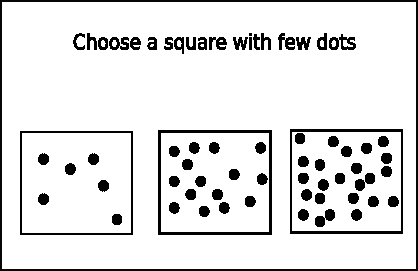
\includegraphics[width=.4\textwidth]{images/stimuluse2}
\caption{An example stimulus from Experiment 2}
\label{stimuluse2}
\end{figure}

The experiment was conducted in a small quiet room.
On arrival in the cubicle, the participant was told that he or she would be presented with objects on screen and required to choose one in response to an instruction on screen, by pressing the button corresponding with the object. There were 5 practice trials. After the practice trials the experimenter left the room. There were 4 blocks of 64 trials each. In between blocks the participant had the opportunity to rest before continuing. The response time dependent variable was measured from the presentation of the squares and dots, until the keypress indicating the participant's choice. The trial would timeout after 60 seconds if there was no response. The dependent variable measuring whether the participant chose the borderline case was also recorded at this time. In this experiment, no feedback was given. This was because, in the vague conditions, we did not regard any response as `correct' or `incorrect', but instead as `borderline response', or `not borderline response', and we did not want to draw participants' attention to this distinction explicitly. We simply recorded whether the participant chose the borderline case or not, and how long it took the participant to respond.

\subsection{Results}

This time around, no responses were treated as erroneous, because errors were essentially undefined for the vague instructions (e.g., `about 10'). It was noted whether participants chose the borderline square. 
%
The RTs were trimmed at 2.5 standard deviations for each subject, leading to the loss of 236 trials, 3.1\% of the data. Means for response times are given in Fig. (\ref{resultse2}).

A linear mixed model was constructed for the response times.
%
Response times were logged; \emph{selection task / instruction format} and \emph{vagueness} were sum-coded and \emph{Item} was centred. 
% 
The fixed effects in the model were \emph{selection task / instruction format} and \emph{vagueness} and their interaction, and \emph{item}.
% 
The random effects in the model were \emph{participant}, and slopes over \emph{participant} for \emph{selection task / instruction format} and \emph{vagueness} and their interaction, and for \emph{item}.

There was a significant effect of \emph{selection task /instruction format} with numerical conditions attracting longer responses than the verbal conditions (numeric: 3284 ms; verbal 1866 ms; a difference of 1418 ms; $\beta=.37, se=.07, t=5.1, p<.001$). 
% 
The effect of \emph{vagueness} was to slow responses down (vague: 2668 ms; crisp: 2450 ms; a difference of 218 ms; $\beta=.06, se=.01, t=4.6, p<.001$). 
%
There was a main effect of \emph{item} ($\beta=.06, se=.008, t=7.0, p<.001$) indicating that response times differed in some way according to which item was presented. However further analysis revealed that there was no consistent smooth trend across items - this effect seems likely to be due to the very fast responses for the smallest item. This item had the largest ratio difference so may have been particularly discriminable for participants. % Reviews asked for an explanation of the difference for numeric crisp over items. Also reviews mention ratio differences as something that we did not control.
%
There was an interaction effect between vagueness and task, such that the disadvantage for vagueness was greater in the numerical than in the verbal instruction conditions ($\beta=-0.13, se= 0.02, t= -6.6, p=0.000$).  [IS THIS CONSISTENT WITH THE ALL-NUMBERS EXPERIMENT 5?]

\begin{figure*}[htbp]
\centering
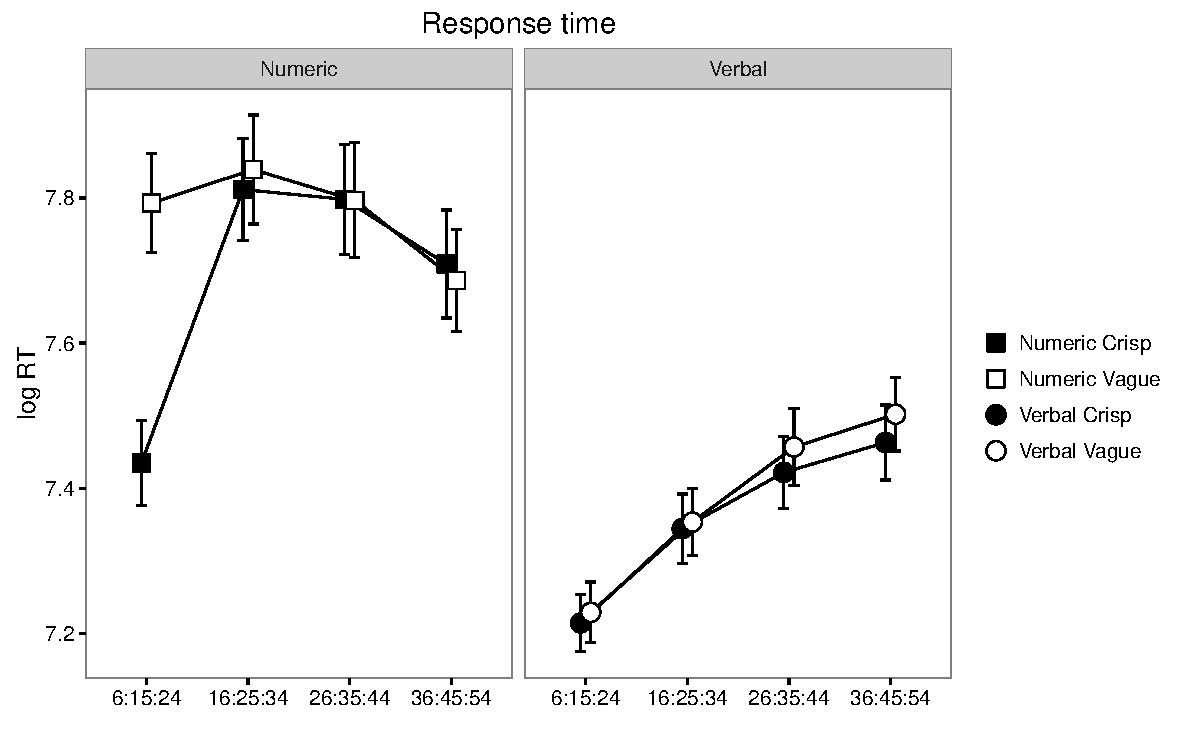
\includegraphics[width=.65\textwidth]{images/response-time-sep-1.pdf}
\caption{Response time results for Experiment 2}
\label{resultse2}
\end{figure*}

Participant grand mean percentage of borderline selections was $16.6\%$. A generalized linear mixed model \cite{jaeger2008categorical} was fit to the data for selection of the borderline response, with task, vagueness and item as fixed effects, and with random slopes for task and vagueness and item over participants.  
%
The distribution of responses over the nearest match square, the borderline square, and the furthest match square are given in Fig, \ref{borderline-response-distribution-e2}.
%
Participants were significantly more likely to choose the borderline option for vague instructions than for precise instructions (21.9\% vs 11.3\%, $\beta=.79, se=.25, z=3.2, p<.01$). Participants were significantly more likely to choose the borderline square when the instruction used the numerical format rather than the verbal format (30.1\% vs 3.0\%, $\beta=3.57, se=.26, z=13.6, p<.001$). 

\begin{figure*}[htbp]
\centering
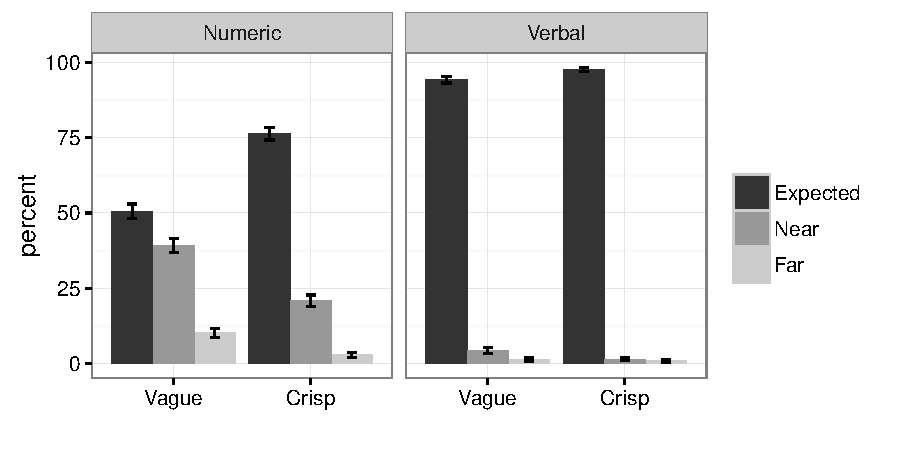
\includegraphics[]{images/histbd4-ggplot-version-1.pdf}
\caption{Distribution of Nearest match, borderline case, and furthest match responses}
\label{borderline-response-distribution-e2}
\end{figure*}


\subsection{Discussion}

This experiment tested to see whether when borderline cases are present, vague instructions would speed responses as they did in Experiment Two when there were no borderline squares. We actually found a \emph{disadvantage} of vague instructions: vague instructions slowed people down by 112 ms on average. We also found that the effect of instruction format was significant, with numerical format slowing responses by 689 ms on average. The disadvantage of numerical format overwhelms the contribution of vagueness. The verbal vague condition was still responded to faster than the numerical crisp condition, so the pattern from Experiment 1 is reproduced, but in the light of the evidence from Experiment 2 in the presence of borderline cases, the advantage that was ascribed to vagueness before now looks more like either an advantage of verbal instruction format, or alternatively as an advantage of the comparison task, according to the selection task account.

% KvD: I've tentatively added the following:
Having effectively separated the {\bf cost reduction} hypothesis from the {\bf instruction format} hypothesis, it is important to observe that, in Experiment 2, instruction format went hand in hand with {\bf selection algorithm}: as shown by the Table of instructions \ref{instructionse2}, the instructions that used a verbal instruction format allowed a comparison algorithm, whereas the instructions that used a numeric format allowed on a matching algorithm. Therefore, our results so far permit the interpretation that what made the instructions in the verbal condition fast is not the fact that they were worded verbally, but that they allowed participants to use a comparison algorithm (which is known to be faster than matching). % KvD I assume we need to say more about this, citing some appropriate papers to support this idea.

In the next two experiments we pitted the comparison and matching selection tasks against each other while controlling vagueness and instruction format. In Experiment 3 we would restrict all the instructions to numeric quantifiers while factorially manipulating vagueness and the comparison / matching selection tasks. In Experiment 4 we would ensure that all instructions used verbal quantifiers, while also factorially manipulating vagueness and the comparison / matching selection tasks. This allows us to distinguish between the predictions of the selection task account and the instruction format account. 

\section{Experiment 3}

\subsection{Introduction}

The main aim of experiment 3 was to see whether vagueness would exert beneficial effects when all conditions used numerals in the instructions, and when there were vague and crisp versions of the instructions for both comparison and matching strategies. The main changes from experiment 2 were that the selection task was explicitly controlled, and that all conditions were constrained to mention a number. We used the same stimuli as in experiment 2. Table \ref{instructionse3} shows the instructions. % KvD I think we should motivate our choice of materials (especially "far ..er")

\begin{table*}[htbp]
\begin{center}
\caption{Experiment 3 Instructions assuming 6,15,24 dots as the Item, and showing fewer instead of more}
\label{instructionse3}
\begin{tabular}{llll}
\toprule
vagueness&instruction format&selection task&instruction\\
\midrule
crisp & numeric&matching & Choose a square with 6 dots \\ 
crisp & numeric&comparison & Choose a square with fewer than 20 dots \\
vague & numeric&matching & Choose a square with about 10 dots \\ 
vague & numeric&comparison & Choose a square with far fewer than 20 dots \\ 
\bottomrule
\end{tabular}
\end{center}
\end{table*}





\subsection{Hypotheses}
% (1) Vague instructions are easier for the reader than crisp alternatives (main effect of vagueness)
%(2) Comparison is easier for the reader than matching (main effect of selection)
%(3) Effects of vagueness are different depending on whether selection is matching or comparison (interaction effect selection x vagueness).

The instruction format account predicts no differences between the conditions, since all conditions used numeric quantifiers.

The selection task account predicts a main effect of selection task such that the comparison conditions would attract faster responses than the matching conditions.

The cost reduction account predicts that there will be a main effect of vagueness such that the vague instruction conditions attract faster responses than the crisp instruction conditions and particularly that at each level of selection task the vague condition should attract faster responses than the crisp condition.


\subsection{Method}

38 volunteers were recruited via internal messaging at University of Aberdeen, with self-reported fluency in English. They were paid ten pounds each for participating.
The apparatus was the same as Experiment 1.
The design was a 2 x 2 factorial manipulation of vagueness and selection task (see Table \ref{instructionse3}).
Each stimulus was an instruction followed by a triple of dots.
First a referring expression instruction was presented. Participants pressed a key to dismiss the instruction and proceed to the squares with dots in them.

\subsection{Results}
A linear mixed effects regression model was built for log response times. The structure of the model was as follows: fixed effects were vagueness, selection task (both sum coded) and centred item and their interactions: random effects were vagueness, selection task, and item (but not their interactions - the model failed to converge when these interactions were included). The means are plotted in Figure \ref{resultse3}.

The results showed that vagueness was beneficial for comparison but detrimental for matching. There was no significant main effect of vagueness ($\beta =.003, se=.014, t=.202, p=.841$). There was a main effect of task type, with the comparison task speeding responses compared to the matching task ($\beta=-.165, se=.027, t=-6.218, p<.001$). Vagueness exerted effects in different directions for the comparison task and for the matching task. Separate analyses were conducted at each level of the selection task to see whether within each task type there were significant effects of vagueness. There were: in the comparison task vagueness significantly speeded response times compared with crisp controls ($\beta=-.07, se=.02, t=3.52, p<.01$). In the matching task vagueness significantly slowed response times compared with crisp controls ($\beta=-.07, se=.02, t=-2.89, p<.05$).

None of the accounts set out in the Hypotheses section emerge well from the results. The instruction format account wrongly predicts no differences between the conditions. The selection task correctly predicted the main effect of selection task, but has no coverage of the interaction with vagueness. The cost reduction account is wrong to predict main effect advantages for vagueness, and wrong to predict that vagueness should be beneficial at each level of the selection task: however vagueness was advantageous in the comparison task.


\begin{figure*}[htbp]
\centering
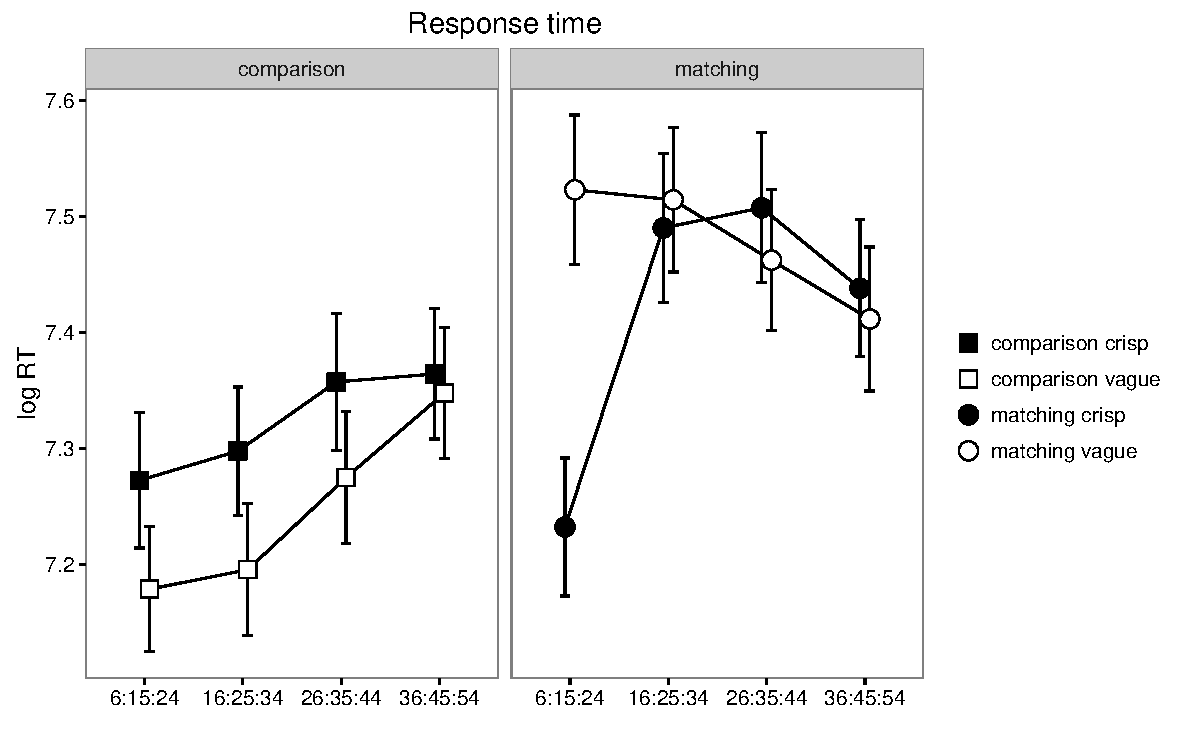
\includegraphics[width=.75\textwidth]{images/response-time-two-panels-1.pdf}
\caption{Results for Experiment 3}
\label{resultse3}
\end{figure*}



\section{Experiment 4}
\subsection{Introduction}
This experiment investigated response times for instructions that did not use a number. 
We manipulated vagueness and the selection task (comparison and matching). 
In order to implement the experiment without mentioning numbers,  we used a prime to visually show the numbers of dots that we wanted to refer to as {\em the target} in the instructions. 
This presentation of a prime before the main trial shares some features with Experiment 2 in \protect \textcite{Izard20081221}, although in that experiment participants were told the numerosity of the prime - called an \emph{inducer} in that paper - in our experiment we did not tell participants the numerosity of the prime array.
An item was thus a combination of a visual prime, a numeric triple, and a referring expression.
The referring expressions were constrained to never mention a numeral, as in Table \ref{Instructions for e4}. 


\begin{table*}[htbp]
\centering
\caption{Experiment 4: Instructions}
\label{Instructions for e4}
\begin{tabular}{lllp{7cm}}
\hline
vagueness&instruction format& selection task&instruction\\
\hline
crisp & verbal&matching & Choose a square with the same number of dots as the target \\ 
crisp & verbal&comparison& Choose a square with fewer dots than the target \\
vague & verbal&matching & Choose a square with about the same number of dots as the target \\ 
vague & verbal&compaison& Choose a square with far fewer dots than the target \\ 
\hline
\end{tabular}
\end{table*}

\subsection{Hypotheses}
The instruction format account predicts no differences between the conditions, since all conditions used verbal quantifiers.

The selection task account predicts a main effect of selection task such that the comparison conditions would attract faster responses than the matching conditions.

The cost reduction account predicts that there will be a main effect of vagueness such that the vague instruction conditions attract faster responses than the crisp instruction conditions and particularly that at each level of selection task the vague condition should attract faster responses than the crisp condition.

\subsection{Method}

40 volunteers recruited via internal messaging at University of Aberdeen, with self-reported fluency in English. They were paid ten pounds for participating. 
The apparatus was the same as Experiment 1.
The design was a 2 x 2 factorial manipulation of vagueness and selection task.
Each stimulus was a sequence of prime, instruction, and squares.
The procedure for this experiment was different from the others, to accommodate the requirement not to use numbers in the instruction. We had to have a different way to indicate a numerosity in the instruction, which we did by adding a visual `prime', a square that contained the number of dots that we wanted to refer to.

\subsection{Results}
The results showed that vagueness was beneficial for comparison but detrimental for matching (the same as Experiment 3) even when no numbers were allowed in the instructions. Figure \ref{resultse4} shows the means by condition. There was no main effect of vagueness ($\beta=.01, se=.01, t=1.51, p=.14$). There was a main effect of selection, with comparison task instructions leading to faster responses than the matching task instructions ($\beta=-.18, se=.02, t=-10.38, p<.01$). This effect was in the same direction as Experiment Four. Vagueness did  exert different effects depending on the selection task ($\beta=.12, se=.03, t=4.32, p<.05$). Separate analyses were conducted for the comparison task and for the matching task. In the comparison task, vagueness resulted in faster response times ($\beta=-0.08, se=.02, t=4.30, p<.05$). In the matching task vagueness slowed response times ($\beta=.05, se=.01, t=3.72, p<.05$). These results are in the same direction as Experiment 3.

\begin{figure*}[htbp]
\centering
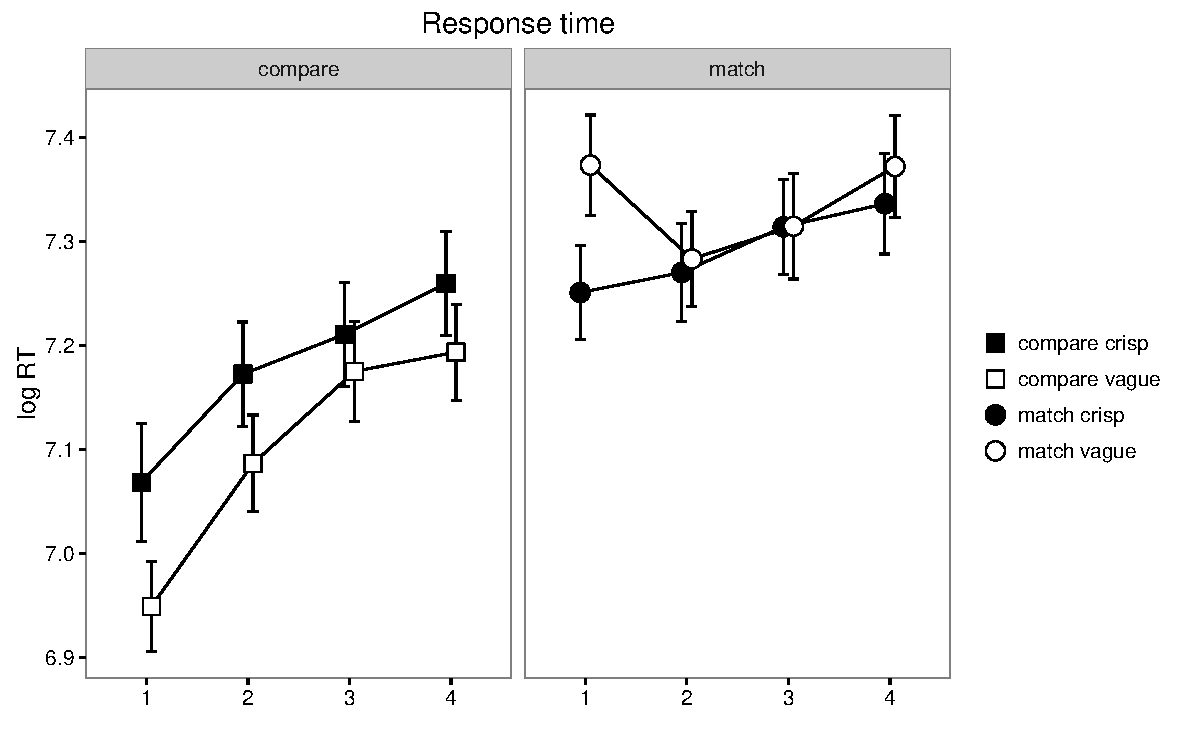
\includegraphics[width=.75\textwidth]{images/response-time-two-panels-1-e4.pdf}
\caption{Results for Experiment 4}
\label{resultse4}
\end{figure*}

Again none of the accounts set out in the Hypotheses section emerge well from the results. The instruction format account wrongly predicts no differences between the conditions. The selection task correctly predicted the main effect of selection task, but has no coverage of the interaction with vagueness. The cost reduction account is wrong to predict main effect advantages for vagueness, and wrong to predict that vagueness should be beneficial at each level of the selection task: however vagueness was advantageous in the comparison task.

\subsection{Discussion of experiments 3 and 4}

The main aim of these two experiments was to test whether vagueness confers any cognitive benefits over and above those due to differences in the selection task according to whether the instruction mandates a \emph{comparison} selection task or a \emph{matching} selection task, when number-use is held constant.  The main effect of selection task showed that the assumption that the \emph{comparison} task is easier than the \emph{matching} task is well-founded. In both experiments people were reliably faster at responding in the \emph{comparison} task. 

Vagueness, which was the phenomenon  on which our investigation focussed, did not exert a main effect in response time. However when the comparison and selection tasks were analysed separately, there was small reliable speedup in RT from the crisp to the vague \emph{comparison} tasks, but a small reliable slowdown in RT from the crisp to the vague \emph{matching} tasks. 

\section{General Discussion}

Experiment 1 showed us that responses were faster and more accurate when the instructions were vague than when they were crisp, but the experiment could not distinguish effects of vagueness from those of number-avoidance or selection task: the vague conditions were also in verbal rather than numerical format; and mandated a comparison strategy rather than a matching strategy.  Experiment 2 showed us that number-avoidance in the verbal format instructions is an important factor driving the faster response times in the task, and that vagueness does not have any additional explanatory power in either the verbal format instructions or the numerical format instructions when we generated verbal and numerical versions of both crisp and vague instructions. However the experiment could not distinguish benefits of number-avoidance in the verbal instructions from benefits of the comparison selection task: the verbal instructions also mandated a comparison strategy rather than a matching strategy. In experiments 3 and 4 we manipulated vagueness and the selection task independently of numerical format. We found that there are effects of the selection task mandated by the instruction, with the comparison task instructions attracting faster response times than the matching instructions, and that vagueness exerts benefits when the selection task is \emph{comparison}, but not when the task is \emph{matching}.

The benefits of vagueness in the \emph{comparison} task in experiments 3 and 4 could be explained as differences in the number of valid targets for the expression, as follows. Taking as an example the stimulus with (6,15,24) dots, it could be argued that the vague comparison instruction (e.g., \emph{a square with far fewer than 20 dots}) has one valid target, the square with 6 dots, while the crisp comparison instruction (e.g., \emph{a square with fewer than 20 dots}) has two valid targets, the squares with 6 and 15 dots. In both experiments 3 and 4 we found that people were quicker to identify a square when the instruction only had one valid target. This leads us to speculate that the benefit for vagueness here could be due to the vague expression foregrounding a particular valid target while the crisp expression carries with it the additional task of distinguishing between two alternative valid targets, something we propose to call a ``range-reduction'' benefit.

What is one entitled to conclude? Given that we were able to identify a class of situations -- namely: situations in which a comparison strategy suffices to identify the intended referent -- in which vague expressions led to faster response times than crisp ones, would it be valid to conclude that we have finally discovered an advantage for vagueness that cannot be ascribed to some other factor? We believe the answer to this question is negative. To see why, consider figures \ref{resultse3} and \ref{resultse4}. Both figures depict four conditions, depending on whether the expression was crisp or vague, and depending on whether the referent could be identified using a comparison strategy or not. Two of the resulting four conditions result in an expression that can denote either of two referents; the other two conditions result in an expression that can only denote one referent, with the other possible referent being a marginal candidate at best:

\begin{table}[htbp]
\caption{Vagueness as range reduction}
\begin{center}
\begin{tabular}{lll}
\hline
vagueness & selection task & candidates\\
\hline
crisp & matching & 1 candidate\\
crisp & comparison & 2 candidates\\
vague & matching & 2 candidates\\
vague & comparison & 1 candidate\\
\hline
\end{tabular}
\end{center}
\label{default}
\end{table}

To see why vagueness thus has opposite effects, depending on whether it is used in matching or comparison situations, compare an instruction like `Choose a square with 6 dots' with its vague counterpart `Choose a square with about 10 dots': by adding the word `about', we broaden the range of squares that the expression might be referring to. On the other hand, compare `Choose a square with fewer than 20 dots' with its vague counterpart `Choose a square with far fewer than 20 dots': by adding the word `far', we did not broaden the range of squares denotable by the expression: we narrow it down, because only some of the squares that have fewer dots may have {\em far} fewer dots.

The observation that conditions with 1 candidate lead to shorter response times than conditions with 2 candidates is consistent with the range reduction hypothesis, but not with the idea that vagueness has a beneficial effect. It appears, in other words, that range reduction causes shorter response times, suggesting that shorter response times will only result from a vague expression if this expression leads to range reduction. Once again, it seems, it is not vagueness itself that has advantages but a phenomenon (namely range reduction) that is an automatic concomitant of vagueness in some types of situations.

The findings from our experiments show that when vague expressions are compared with crisp alternatives in our forced choice task, vague expressions appear to yield benefits in some situations, but that the observed benefits may be due to factors other than vagueness itself that the vague forms bring along with them: factors like avoiding numbers; permitting comparison tasks; and range reduction. The picture that is starting to emerge, in other words, is subtle: on the one hand, in the situations that we have been studying -- where cooperative speakers refer to an object (e.g., a square) by means of some quantity associated with the object (e.g., the number of dots contained in the square) -- vagueness is not intrinsically beneficial. On the other hand, vague expressions often have other features that {\em are} beneficial, and these are what give us the incorrect impression that vagueness itself is beneficial. Vagueness may thus have acquired a reputation that it does not deserve. 

A comparison may clarify the logic of the situation. In recent years a number of studies, focussing typically on red wine, have suggested that alcohol, consumed in low doses, may have health benefits. An alternative explanation, however, asserts that it is not the alcohol in the wine that is beneficial, but the antioxidants from grapes. If this alternative explanation is correct then alcohol may not be as beneficial as some of us would have it. % KvD Good hey?


\printbibliography

\appendix
\section{}

Table \ref{AllInstructions} shows the relevant properties of all the experiments in a single view.

\newgeometry{bottom=2cm}

\newcommand\T{\rule{0pt}{2.6ex}}       % Top strut
\newcommand\B{\rule[-2.2ex]{0pt}{0pt}} % Bottom strut

\begin{sidewaystable}
\caption{All Instructions}
\label{AllInstructions}

    \resizebox{\linewidth}{!}{%
    \begin{tabular}{clcccccc}
%    \midrule
    $E$&Example instruction&$V$&$Q$&Symmetry&Algorithm&$N$&Def\\
       \toprule
    1&Choose the square with 5 dots&Crisp&Number&Symmetric&Matching&1&Definite\\
    1&Choose the square with few dots&Vague&Word&Asymmetric&Comparison&1&Definite\B\\
%    \midrule
%\rule{0pt}{0cm} \\
    2&Choose the square with 6 dots&Crisp&Number&Symmetric&Matching&1&Definite\\
    2&Choose a square with about 10 dots&Vague&Number&Symmetric&Matching&2&Indefinite\\
    2&Choose the square with the fewest dots&Crisp&Word&Asymmetric&Comparison&1&Definite\\
    2&Choose a square with few dots&Vague&Word&Asymmetric&Comparison&2&Indefinite\B\\
%    \midrule
    3&Choose a square with 6 dots&Crisp&Number&Symmetric&Matching&1&Indefinite\\
    3&Choose a square with fewer than 20 dots&Crisp&Number&Asymmetric&Comparison&2&Indefinite\\
    3&Choose a square with about 10 dots&Vague&Number&Symmetric&Matching&2&Indefinite\\
    3&Choose a square with far fewer than 20 dots&Vague&Number&Asymmetric&Comparison&1&Indefinite\B\\
%    \midrule
    4&Choose a square with the same number of dots as the target&Crisp&Word&Symmetric&Matching&1&Indefinite\\
    4&Choose a square with fewer dots than the target&Crisp&Word&Asymmetric&Comparison&2&Indefinite\\
    4&Choose a square with about the same number of dots as the target&Vague&Word&Symmetric&Matching&2&Indefinite\\
    4&Choose a square with far fewer dots than the target&Vague&Word&Asymmetric&Comparison&1&Indefinite\\
    \bottomrule
    \end{tabular} 
    }
    ~\\
    E:~Experiment number\\
    $V$:~Vagueness\\
    $Q$:~Quantifier used\\
%    Symmetry:~\\
%    Algorithm:~\\
     $N$:~Number of valid targets for the instruction\\
     Def:~Definiteness of the article in the instruction: a/the
   
\end{sidewaystable}



\end{document}

%%%%%%%%%%%%%%%%%%%%%%%%%%%%%%%%%%%%%%%%%%%%%%%%%%%%
%%%%%%%%%%%%%%%%%%%%%%%%%%%%%%%%%%%%%%%%%%%%%%%%%%%%



\section{}


\end{document}


%\begin{figure*}
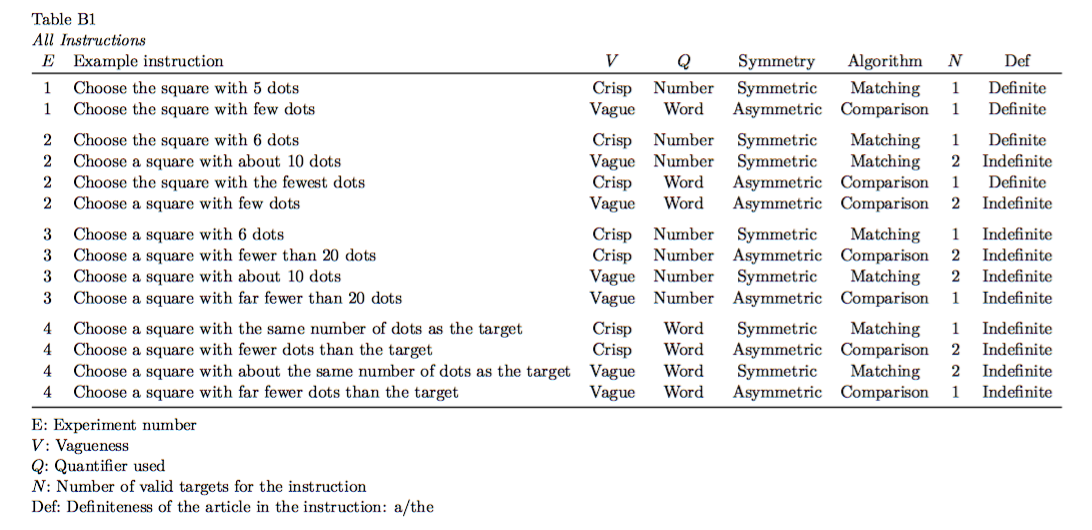
\includegraphics[angle=90,origin=c, scale=.5]{images/appendix_table}
%\end{figure*}

